\section{Optimización en redes: El problema de flujo con coste mínimo}

\subsection{Introducción}

Los problemas de flujos en redes (tipo especial de los de transporte) permiten flujos que usan puntos intermedios o
de transbordo, y es característico el uso de arrays dispersos asociados a los arcos de un grafo no completo. Abarcan áreas
diversas como la producción, distribución y planificación de proyectos, localización de instalaciones, administración
de recursos y gestión de inversores entre otras. El problema más importante de optimización en redes es el problema de
flujo de costo mínimo.

\subsection{Terminología}

Un grafo consiste en un conjunto de puntos y un conjunto de líneas que unen unos pares de puntos. Siendo específicos, un
grafo está formado por \textbf{nodos} (los puntos) y \textbf{arcos o aristas} (las líneas). Por tanto, un grafo es un par
$(N,A)$ donde $N$ es un conjunto de nodos y $A$ un conjunto de arcos que relacionan los elementos de $N$. Un grafo puede
estar diseñado para permitir el paso de algún flujo, como puede ser la red de carreteras nacionales, un sistema de tuberías
o la block-chain (flujos de monedas entre carteras). Si el flujo se permite en una sola dirección se dirá que se trata de
un \textbf{arco dirigido}, en caso contrario será un \textbf{arco no dirigido}. Cuando una red solo tiene arcos no dirigidos
se habla de una \textbf{red dirigida} (como podráin ser las tuberías), así mismo y como se podría suponer, cuando una red
solo tiene arcos no dirigidos, se tratará de una \textbf{red no dirigida}. Toda red podrá considerarse dirigida sustituyendo
los arcos no dirigidos por un par de arcos dirigidos con direcciones opuestas.

\vspace*{2mm}

Una trayectoria entre dos nodos es la sucesión de arcos distintos que conectan ambos nodos. Cuando algunos o todos los
arcos de una red son arcos dirigidos, distinguiremos entre trayectorias dirigidas y trayectorias no dirigidas. Una 
\textbf{trayectoria dirigida o camino} del nodo $i$ al nodo $j$ es una sucesión de arcos cuya dirección es hacia el nodo 
$j$; de la misma forma, una \textbf{trayectoria no dirigida o cadena} del nodo $i$ al nodo $j$ es una sucesión de arcos
cuya dirección (si la tienen), es hacia o desde el nodo $j$.

\begin{center}
    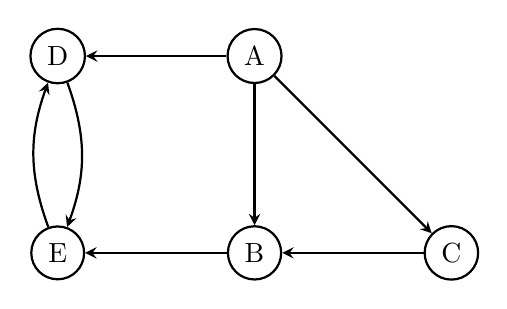
\begin{tikzpicture}[->, >=stealth, node distance=2.5cm, thick]
        % Nodos
        \node[circle, draw] (A) {A};
        \node[circle, draw, below of=A] (B) {B};
        \node[circle, draw, left of=B] (E) {E};
        \node[circle, draw, right of=B] (C) {C};
        \node[circle, draw, left of=A] (D) {D};
    
        % Aristas dirigidas
        \draw (A) -- (B);
        \draw (A) -- (C);
        \draw (A) -- (D);
        \draw (C) -- (B);
        \draw (B) -- (E);
        \draw[bend left=20] (D) to (E);
        \draw[bend left=20] (E) to (D);
    \end{tikzpicture}
\end{center}

Este grafo (red) está definidos por el conjunto de nodos $N=\{A,B,C,D,E\}$ y el conjunto de arcos 
$A={(A,B),(A,C),(A,D),(B,E),(C,B),(D,E),(E,D)}$. La sucesión de arcos $\{(C,B),(B,E),(E,D)\}$ es una trayectoria dirigida del
nodo $C$ al nodo $D$.

\newpage

\subsection{Problema del flujo de coste mínimo}

Sea $G=(N,A)$ un grafo dirigido con un conjunto de nodos $N=\{1,\dots,m\}$ y un conjunto de arcos $A$ representados por pares
$(i,j)$ con $i,j\in N$. La red corresponiende al grafo $G$ tiene los siguientes elementos adicionales.

\begin{itemize}
    \item Asociado a cada nodo $i\in N$ se tiene una cantidad $b_i$ que representa la oferta o demanda de cierto producto
          en ese nodo. Si $b_i>0$ se dice que el nodo es un \textbf{nodo oferta}, con un nivel de oferta (existencias o 
          producción) de $b_i$. Si $b_i<0$ entonces se dice que es un \textbf{nodo demanda}. Finalmente, si $b_i=0$ será
          un \textbf{nodo intermedio o de transbordo}.
    \item Para cada nodo $i\in N$ consideramos los conjuntos de nodos $\partial_i^+$ y $\partial_i^-$ donde 
          $\partial_i^+=\{j\in N:(i,j)\in A\}$ y $\partial_i^-=\{j\in N:(j,i)\in A\}$, representando al conjunbto de arcos
          ``salientes'' y ``entrantes'' respectivamente (a los que se llega desde $i$ y desde los que se llega a $i$).
    \item Asociado a cada arco una variable $x_{ij}\geq0$, que representa la cantidad de producto o flujo sobre el arco $(i,j)$
    \item Asi mismo, será $c_{ij}$ el coste por unidad del producto transportada a lo largo del arco.
    \item En ocasiones se establece $u_{ij}$ como la capacidad de flujo sobre el arco $(i,j)$.
\end{itemize}

\noindent La formulación del problema es la siguiente

\begin{alignat}{3}
    \text{minimizar:}   & \quad & \sum_{(i,j)\in A}c_{ij}x_{ij}                                     & \quad &                               \\
    \text{sujeto a:}    & \quad & \sum_{j\in \partial_i^+}x_{ij}-\sum_{j\in \partial_i^-}x_{ij}=b_i &       & \forall i\in N \label{eq:35}  \\
                        & \quad & x_{ij}\geq 0                                                      &       & \forall (i,j)\in A     
\end{alignat}

A las restricciones definidas en \ref{eq:35} se conocen como las \textit{ecuaciones de conservación de flujo}, 
\textit{ecuaciones de balance} o las \textit{ecuaciones de Kirchoff}. Hacen referencia al balance de los flujos de entrada
(aristas que vienen de los nodos $\partial_i^+$) y los flujos de salida (aristas que van a los nodos $\partial_i^-$) y el 
``consumo'' (o la ``emisión'') local definida por $b_i$.

\vspace*{2mm}

Si el número de arcos en el grafo es $n$ y representamos por $x=(x_{ij})$ al vector de variables o flujos, por $c=(c_{ij})$
al vector de costes y $b=(b_{i})$ el vector de ``balances'', el problema puede formularse de forma matricial como sigue

\begin{alignat}{3}
    \text{minimizar:}   & \quad & cx                & \quad &   \\
    \text{sujeto a:}    & \quad & Ax=b              &       &   \\
                        & \quad & x\geq \mathbf{0}  &       &        
\end{alignat}

donde $A$ es la matriz de coeficientes de las ecuaciones de balance. La variable $x_{ij}$ asociada al arco $(i,j)\in A$
aparecerá con coeficiente 1 en la restricción correspondiente al nodo $i$ y con coeficiente -1 en la restricción correspondiente
al nodo $j$. La matriz $A$ es conocida como \textit{matriz de incidencias nodos-arcos} para un grafo dirigido cualquiera.

\newpage

\begin{ejemplo}
    Para el grafo dado por el conjunto de nodos $N=\{1,2,3,4\}$ y el conjunto de arcos 
    $A=\{(1,2),(1,2),(2,3),(2,4),(3,2),(3,4),(4,1)\}$ la matriz de restricciones es la matriz de incidencias nodos-arcos

    \[A=\begin{pmatrix}
         1 &  1 &  0 &  0 &  0 &  0 & -1 \\
        -1 &  0 &  1 &  1 & -1 &  0 &  0 \\
         0 & -1 & -1 &  0 &  1 &  1 &  0 \\
         0 &  0 &  0 & -1 &  0 & -1 &  1
    \end{pmatrix}\]

    \noindent El arco $(1,2)$ une desde el nodo 1 al nodo 2, por lo que $a_{11}=1$ y $a_{12}=-1$, del mismo modo ocurre con 
    el resto de arcos. Como hay 4 nodos y 7 arcos las dimensiones de $A$ son $7\times 4$.
\end{ejemplo}

El modelo de flujos de redes tiene una propiedad importante, la \textbf{propiedad de integralidad} (no confundir con 
\textit{integrabilidad}). Esta propiedad puede enunciarse como ``si las ofertas y demandas son números enteros, toda solución
básica factible tiene valores enteros''. Es por esto que los problemas de flujo en redes muchas veces se incluyen en los
estudios del campo de la programación entera (como en nuestra asignatura).

\subsection{Redes balanceadas}

Se define la oferta total como la cantidad positiva $O_T=\sum_{b_i>0}b_i$, osea la suma de las ofertas. Del mismo modo,
se define la demanda total como la cantidad positiva $D_T=-\sum_{b_i<0}b_i$. Diremos que una red está balanceada si la oferta
es igual a la demanda, esto es $O_T=D_T$, o dicho de otra forma, si $\sum_ib_i=0$. Para todo problema factible su red está
balanceada, pero no toda red balanceada genera un problema factible.

\vspace*{2mm}

En muchos casos prácticos sucede que la oferta total no coincide con la demanda totaly es necesario ajustar el
problema para convertirlo en una red balanceada. Para ello se pueden asignar restricciones en función de si un nodo es de
oferta o de demanda, pero en la práctica esto resulta muy incomodo. Lo habitual es añadir un nodo ficticio conectado con arcos
dirigidos a todos los demás con coste 0 y demanda $D_T-O_T<0$

\subsection{Extensiones y aplicaciones}

En los problemas de redes, los costes y capacidades están siempre asociados a los arcos. En ocasiones, se quiere o necesita
establecer alguna de estas caracteristicas a un nodo (costes de fabricación, etc) por lo que se ha de crear un arco ficticio
que desdoble al nodo donde se adjudiquen estas características. Otra posible variante es incluir cotas mínimas, cambiando
las restricciones a $l_{ij}\leq x_{ij}\leq u_{ij}$.

\vspace*{2mm}

Existen otros problemas que generalizan el modelo básico y que tienen gran cantidad de aplicaciones en distintos sectores. A
pesar de que no se estudiarán, se enuncian algunos

\begin{itemize}
    \item Redes Generalizadas (tambien conocidas como Redes con Pérdidas y Ganancias)
    \item Redes Multiproducto
    \item Redes con costos fijos (se estudian en el tema de programación entera)
    \item Redes no lineales (cuando la función objetivo no es lineal)
\end{itemize}

Las aplicaciones más importantes de lo problemas de flujo en redes se dan en \textit{problemas de distribución}, pero tienen
impacto en ambitos como la planificación de \textit{redes espacio/tiempo} para modelizar problemas de producción/inventario.